\documentclass[11pt]{elegantbook}
\usepackage{graphicx}
\usepackage{float}
\definecolor{structurecolor}{RGB}{40,58,129}
\linespread{1.6}
\setlength{\footskip}{20pt}
\setlength{\parindent}{0pt}
\newcommand{\argmax}{\operatornamewithlimits{argmax}}
\newcommand{\argmin}{\operatornamewithlimits{argmin}}
\elegantnewtheorem{proof}{Proof}{}{Proof}
\elegantnewtheorem{claim}{Claim}{prostyle}{Claim}
\DeclareMathOperator{\col}{col}
\title{Optimization}
\author{Wenxiao Yang}
\institute{Haas School of Business, University of California Berkeley}
\date{2023}
\setcounter{tocdepth}{2}
\extrainfo{All models are wrong, but some are useful.}

\cover{cover.jpg}

% modify the color in the middle of titlepage
\definecolor{customcolor}{RGB}{32,178,170}
\colorlet{coverlinecolor}{customcolor}
\usepackage{cprotect}

\addbibresource[location=local]{reference.bib} % bib

\begin{document}
\maketitle

\frontmatter
\tableofcontents

\mainmatter

\chapter{Extreme Value and Coercive Functions}

\section{Bolzano-Weierstrass theorem}
\subsection{Sequence Convergence}
\begin{definition}[Sequence Convergence]
    A sequence $\vec{x}_1,\vec{x}_2,\vec{x}_3,...$ of points converges to $\vec{x}^*$ if for any $\varepsilon>0$, there exists some integer $n\in \mathbb{N}$ such that $$\|\vec{x}_m-\vec{x}^*\|<\varepsilon,\ \forall m\geq n$$
\end{definition}

\subsection{Bolzano-Weierstrass Theorem: Compact set $S$, $\exists$ subsequence converges to $\vec{x}^*\in S$}
\begin{theorem}[Bolzano-Weierstrass]
    Let $S\subseteq \mathbb{R}^n$ be a compact (closed and bounded) set and let $\vec{x}_1,\vec{x}_2,...$ be any sequence of points in $S$.\\
    Then we can choose a subsequence of points that has a limit $\vec{x}^*\in S$. Formally, we can choose indices $i_1<i_2<i_3<\cdots$ such that the sequence $\vec{x}_{i_1},\vec{x}_{i_2},\vec{x}_{i_3},...$ converges to $\vec{x}^*\in S$.
\end{theorem}
\begin{enumerate}[$\bullet$]
        \item "$S$ is bounded" $\Rightarrow$ we can choose a subsequence $\vec{x}_{i_1},\vec{x}_{i_2},\vec{x}_{i_3},...$ converges to $\vec{x}^*\in S$.
        \item "$S$ is closed" $\Rightarrow$ the limit of this subsequence is \underline{in} $S$.
\end{enumerate}

\subsection{Extreme Value Theorem: continuous $f$ compact set $\rightarrow \mathbb{R}$ has global-min/max}
\begin{corollary}[Extreme value theorem]
    If $S\subseteq \mathbb{R}^n$ is a \textbf{compact} (closed and bounded) set and $f: S \rightarrow \mathbb{R}$ is a continuous function, then $f$ has a global maximizer/minimizer on $S$.
\end{corollary}


\subsection{Corollary: Non-empty and Compact level set $\{x \mid f(x) \leq c\}$ $\Rightarrow$ $\exists$ $f$'s global-min/max}

\begin{corollary}[bounded level sets]
    Suppose $f: \mathbb{R}^{d} \rightarrow \mathbb{R}$ is a continuous function. If for a certain $c$, the level set
    $$
    \{x \mid f(x) \leq c\}
    $$
    is \textbf{non-empty} and \textbf{compact}, then the global minimizer of $f$ exists, i.e., there exists $x^{*} \in \mathbb{R}^{d}$ s.t.
    $$
    f\left(x^{*}\right)=\inf _{x \in \mathbb{R}^{d}} f(x)
    $$
\end{corollary}
\begin{example}
    $f(x) = x^2$.
    Level set $\{x|x^2 \leq 1\}$ is $\{x|-1\leq x\leq 1\}$: non-empty compact. Thus, there exists a global minimum.
\end{example}
\section{Coercive function}
\subsection{Def: Coercive function}
\begin{definition}
    A continuous function $f: \mathbb{R}^n \rightarrow \mathbb{R}$ is \textbf{coercive} if for all $c\in \mathbb{R}$, the \textbf{subset set} $\{x | f(x) \leq c\}$ is bounded.
\end{definition}
(all level sets bounded $\Leftrightarrow$ coercive): Let $f$ be a continuous function, then $f$ is coercive iff $\{x | f(x) \leq \alpha\}$ is compact for any $\alpha$.

Coercive $\Rightarrow$ one non-empty bounded level set; but not the other way.

\subsection{Coercive function $f$ $\Rightarrow$ $\exists$ global-min}
\begin{corollary}[coercive]
    Suppose $f: \mathbb{R}^{d} \rightarrow \mathbb{R}$ is a continuous function. If $f$ is coercive ($f(x) \rightarrow \infty$ as $\|x\| \rightarrow \infty$), then the global minimizer of $f$ over $\mathbb{R}^{d}$ exists.
\end{corollary}
\begin{proof}
Let $\alpha\in \mathbb{R}^d$ be chosen so that the set $S = \{x |f(x) \leq \alpha\}$ is non-empty. By coercivity,
this set is compact. Then, by the extreme value theorem, we have the global minimer.
\end{proof}

\subsection{Lemma: $f: \mathbb{R}^n \rightarrow  \mathbb{R}$ is coercive $\Leftrightarrow$ $\lim_{\|\vec{x}\| \rightarrow \infty}f(\vec{x})=+\infty$ for all possible directions.}
\begin{lemma}
    Coercive $f: \mathbb{R} \rightarrow \mathbb{R}$ $\Leftrightarrow$ $\lim_{x \rightarrow +\infty}f(x)=\lim_{x \rightarrow -\infty}f(x)=+\infty$\\
    More generally, $f: \mathbb{R}^n \rightarrow  \mathbb{R}$ is coercive $\Leftrightarrow$ $\lim_{\|\vec{x}\| \rightarrow \infty}f(\vec{x})=+\infty$ for all possible directions.
\end{lemma}

\subsection{Lemma: sum of \textit{coercive functions} is a coercive function}
\begin{lemma}
    If $f_1,f_2,...,f_n$ are coercive functions $\mathbb{R} \rightarrow  \mathbb{R}$, then $f(\vec{x})=\sum_{i=1}^n f_i(x_i)$ is coercive.
\end{lemma}

\subsection{Lemma: \textit{coercive function} $+$ \textit{bounded below function} is a coercive function}
\begin{lemma}
    If $f: \mathbb{R}^n \rightarrow \mathbb{R}$ is coercive, and $g: \mathbb{R}^n \rightarrow \mathbb{R}$ is continuous and bounded below, then $f+g$ is coercive.
\end{lemma}
Some special cases of this lemma:
\begin{enumerate}[$\bullet$]
    \item Since coercive functions have global minimizers, they are always bounded below, so in particular, the sum of two coercive functions is coercive.
    \item If $f$ is coercive and $h$ is a continuous function such that $f(x) \leq h(x)$ for all $x$, then $h = f + g$, where $g = f - h$, and $g$ is bounded below (by $0$), so $h$ is also coercive.
\end{enumerate}

\subsection{Get coercive function: convex $f$, $f^\varepsilon(\vec{x})=f(\vec{x})+\varepsilon\|\vec{x}\|^2$ is coercive}
\begin{lemma}
If $f: \mathbb{R}^n \rightarrow \mathbb{R}$ is a convex function, then $f^\varepsilon$ is both convex and coercive for all $\varepsilon>0$.
\end{lemma}

\section{Polynomials Coercive}
\subsection{Quadratic forms: $A_{n\times n}$ is positive definite $\Leftrightarrow$ quadratic form $f(\vec{x})=\vec{x}^TA \vec{x}$ is coercive}
\begin{theorem}
    $A$ is $n\times n$ positive definite $\Leftrightarrow$ quadratic form $f(\vec{x})=\vec{x}^TA \vec{x}$ is coercive.
\end{theorem}
\begin{proof}
    Let $S$ be the set $\left\{\vec{x} \in \mathbb{R}^n:\|\vec{x}\|=1\right\} . S$ is closed and bounded, so $f(\vec{x})$ has a global minimizer $\vec{x}^*$ on $S$. Let $\alpha=f\left(\vec{x}^*\right)$.

    Fun fact: actually $\alpha$ is the smallest eigenvalue of $A$. But we don't need to know that. All we need to know is that $\alpha=\vec{x}^{* \top} A \vec{x}^*>0$, because $A$ is positive definite, and that for all $\vec{x}$ with $\|\vec{x}\|=1$, $f(\vec{x}) \geq \alpha$.
    Now take an arbitrary $\vec{x} \in \mathbb{R}^n, \vec{x} \neq \vec{0}$. We have
    $$
    f(\vec{x})=\vec{x}^{\top} A \vec{x}=\left(\frac{\vec{x}}{\|\vec{x}\|}\right)^{\top} A\left(\frac{\vec{x}}{\|\vec{x}\|}\right) \cdot\|\vec{x}\|^2 \geq \alpha \cdot\|\vec{x}\|^2 .
    $$
    We can show that $\alpha\|\vec{x}\|^2$ is a coercive function, because the sublevel set $\left\{\vec{x} \in \mathbb{R}^n: \alpha\|\vec{x}\|^2 \leq c\right\}$ is the disk around $\vec{0}$ of radius $\sqrt{\frac{c}{\alpha}}$, which is bounded.
    
    Since $f(\vec{x}) \geq \alpha\|\vec{x}\|^2$ for all $\vec{x}$ (including $\vec{0}$, because both functions are 0 there), we know that $f$ is a coercive function as well.
    
    In fact, this condition goes both ways: if $A$ is a symmetric matrix, then $\vec{x}^{\top} A \vec{x}$ is only coercive when $A$ is positive definite. If not, then we can find a nonzero $\vec{y}$ for which $\vec{y}^{\top} A \vec{y} \leq 0$; for any scalar $t$, we'll have $(t \vec{y})^{\top} A(t \vec{y}) \leq 0$, so the sublevel set $\left\{\vec{x}: \vec{x}^{\top} A \vec{x}\right\}$ will contain an entire unbounded line $\{t \vec{y}: t \in \mathbb{R}\}$.
\end{proof}

\subsection{Higher-degree polynomials}
The leading term is the one that will affect the behavior as $x \rightarrow \pm \infty$.
\begin{enumerate}[$\bullet$]
    \item If the leading term has \underline{odd} degree, then the polynomial will be positive in one direction and negative in the other; such polynomials can \underline{never} be coercive.
    \item If the leading term has \underline{even} degree, the polynomial is coercive if and only if the coefficient of the leading term is \underline{positive}.
\end{enumerate}
\begin{theorem}
    A polynomial $f(x, y, z)$ is coercive if both of the following hold:
    \begin{enumerate}[(1)]
        \item It contains $x^A, y^B, z^C$ terms with positive coefficients, where $A, B, C$ are some even integers.
        \item For every other term $x^a y^b z^c$ (with any coefficient) that could potentially be negative, we have $\frac{a}{A}+\frac{b}{B}+\frac{c}{C}<1$.
    \end{enumerate}
\end{theorem}
\begin{proof}
    If $\frac{a}{A}+\frac{b}{B}+\frac{c}{C}<1$, then we can choose positive real numbers $A^{\prime}<A, B^{\prime}<B$, and $C^{\prime}<C$ such that $\frac{a}{A^{\prime}}+\frac{b}{B^{\prime}}+\frac{c}{C^{\prime}}=1$.
Now apply the AM-GM inequality: $\frac{a}{A^{\prime}} x^{A^{\prime}}+\frac{b}{B^{\prime}} y^{B^{\prime}}+\frac{c}{C^{\prime}} z^{C^{\prime}} \geq x^a y^b z^c$.
This holds only for $x, y, z \geq 0$, but we can extend it to all $x, y, z$ by replacing them with $|x|,|y|,|z|$ on the left-hand side. We really want the negation of this, though:
$$
-\frac{a}{A^{\prime}}|x|^{A^{\prime}}-\frac{b}{B^{\prime}}|y|^{B^{\prime}}-\frac{c}{C^{\prime}}|z|^{C^{\prime}} \leq-\left|x^a y^b z^c\right| \leq x^a y^b z^c .
$$
So we can replace the $x^a y^b z^c$ term with $|x|^{A^{\prime}},|y|^{B^{\prime}}$, and $|z|^{C^{\prime}}$ terms (with negative coefficients, but we don't care about coefficients here). This only makes the function smaller. Therefore, if the resulting function is coercive, so was the original.

After we do replace all such mixed terms (and drop any mixed terms that are always nonnegative, such as $x^2 y^2 z^2$ ), we have a sum of functions of $x, y$, and $z$. These are all coercive and therefore so is their sum. For example, the function of $x$ has an $x^A$ term, and some lower-order terms with $|x|^{A^{\prime}}$ for some $A^{\prime}<A$, so $x^A$ (which is coercive) determines its behavior.
\end{proof}

This condition is \underline{sufficient, but not necessary}. If we allow terms $x^a y^b z^c$ with $\frac{a}{A}+\frac{b}{B}+\frac{c}{C}=1$, sometimes the function we get is still coercive. But then, the coefficients start to matter: for example, by the theorem about quadratic forms, $x^2+x y+y^2$ is coercive but $x^2+3 x y+y^2$ is not. This can get tricky.


\chapter{Unconstrained Optimization}
Function: $f:\mathbb{R}^n \rightarrow	\mathbb{R}^n$, $x\in \&,\ \&\subseteq \mathbb{R}^n$.

Terminology: $x^*$ will always be the optimal input at some function.

\section{Basic Definitions}
\subsection{Optimization in a Set}
$$\begin{array}{ll}\text { minimize } & f(x) \\ \text { subject to } & x \in X\end{array}$$
- Objective function $f: \mathbb{R}^{n} \rightarrow \mathbb{R}$ is a continuous function

- Optimization variable $x \in X$

- Local minimum of $f$ on $X: \exists \epsilon>0$ s.t. $f(x) \geq f(\hat{x})$, for all $x \in X$ such that $\|x-\hat{x}\| \leq \epsilon$;

i.e., $x^{*}$ is the best in the intersection of a small neighborhood and $X$

- Global minimum of $f$ on $X: f(x) \geq f\left(x^{*}\right)$ for all $x \in X$

"Strict global minimum", "strict local minimum" "local maximum", "global maximum" of $f$ on $X$ are defined accordingly

\subsection{Minimizer}
\begin{definition}
    \quad\\
    Say $x^*$ is a \underline{global minimizer(minimum)} of $f$ if $f(x^*)\leq f(x), \forall x\in \&$.

    Say $x^*$ is a \underline{unique global minimizer(minimum)} of $f$ if $f(x^*)< f(x), \forall x\neq x^*$.

    Say $x^*$ is a \underline{local minimizer(minimum)} of $f$ if $\exists r>0$ so that $f(x^*)\leq f(x)$ when $\|x-x^*\|<r$.
\end{definition}

A minimizer is \underline{strict} if $f(x^*)< f(x)$ for all relevant $x$.

\subsection{Stationary Point, Saddle Point}
All points $x^*$ s.t. $\nabla f(x^*)=0$ are called \underline{stationary points}.

Thus, all extrema are stationary points.

But not all stationary points have to be extrema.

\underline{Saddle points} are the stationary points neither local minimum nor local maximum.

\begin{example}
$f(x)=x^3$, $x=0$ is a stationary point but not extrema. (saddle point)
\end{example}

\subsection{Conditions for Global Minimizer: (1) exists global-minimizer; (2) has the minimum value in all stationary points}
\begin{claim}
    Consider a differentiable function $f$. Suppose:
    \begin{enumerate}[(C1)]
        \item $f$ has at least one global minimizer;
        \item The set of stationary points is $S$, and $f\left(x^{*}\right) \leq f(x), \forall x \in S$.
    \end{enumerate}
    Then $x^{*}$ is a global minimizer of $f^{*}$.
\end{claim}

\begin{proof}
Suppose $\hat{x}$ is a global minimizer of $f$, i.e.,
$$
f(\hat{x}) \leq f(x), \forall x .
$$
By the necessary optimality condition, we have $\nabla f(\hat{x})=0$, thus $\hat{x} \in S$. By (C2), we have
$$
f\left(x^{*}\right) \leq f(\hat{x}) .
$$
Combining the two inequalities, we have $f(\hat{x}) \leq f\left(x^{*}\right) \leq f(\hat{x})$, thus $f(\hat{x})=f\left(x^{*}\right)$. Plugging into the second inequality, we have $f\left(x^{*}\right) \leq f(x), \forall x$. Thus $x^{*}$ is a global minimizer of $f^{*} .$
\end{proof}

\section{Special Situation: Optimization in $\mathbb{R}$}
\subsection{Necessary condition of local-min: $f'(x^*)=0$}

\begin{theorem}
If $f(x)$ is differentiable function on interval $I$ and $x^*$ is a local minimizer, then either $x^*$ is an endpoint of $I$ or $f'(x^*)=0$.
\end{theorem}

\begin{proof}
Suppose $x^*$ is a local-min of $f$ and not an endpoint of $I$.

Def of $f'(x)=\lim_{h \rightarrow 0} \frac{f(x+h)-f(x)}{h}$\\
Def of local minimizer: $f(x^*)-f(x)\geq 0, |x^*-x|<r$\\
when $0<h<r$, $\frac{f(x+h)-f(x)}{h}\geq 0$; when $-r<h<0$, $\frac{f(x+h)-f(x)}{h}\leq 0$. Then $f'(x)=0$.
\end{proof}

\subsection{Sufficient condition of local-min: $f'(x^*)=0, f''(x^*)\geq 0$}

\subsection{Sufficient condition of global-min: $f'(x^*)=0$ and $f''(x)\geq 0,\forall x\in I$}
\begin{theorem}
    If $f:\mathbb{R} \rightarrow \mathbb{R}$ is a function with a continuous second derivative and $x^*$ is a critical (stationary) point of $f$ (i.e. $f'(x)=0$), then:\\
    (1): If $f''(x)\geq 0,\ \forall x\in\mathbb{R}$, then $x^*$ is a global minimizer on $\mathbb{R}$.\\
    (2): If $f''(x)\geq 0,\ \forall x\in[a,b]$, then $x^*$ is a global minimizer on $[a,b]$.\\
    (3): If we only know $f''(x^*)\geq 0$, $x^*$ is a local minimizer.
\end{theorem}
\begin{proof}
\quad\\
(1)$f(x)=f(x^*)+f'(x^*)(x-x^*)+\frac{1}{2}f''(\xi)(x-x^*)^2=f(x^*)+0+\textit{something non negative}\geq f(x^*)\  \forall x$\\
(2) Similar to (1)\\
(3)$f''(x^*)\geq 0,\ f''$ continuous $\Rightarrow \exists r$ s.t. $f''(x)\geq 0$ $\forall x\in[x^*-\frac{r}{2},x^*+\frac{r}{2}]$, then $x$ is a local minimizer.
\end{proof}

\section{Restriction to a Line}
We want to use a way to represent how a point changes along a specific direction.
\subsection{Definition: $\phi_{\vec{u}}(t)=f(\vec{x}+t\vec{u}),\ \vec{x},\vec{u}\in \mathbb{R}^n, t\in \mathbb{R}$}
\begin{definition}
    Given a point $\vec{x}\in \mathbb{R}^n$ and a direction vector $\vec{u}\neq 0, \in \mathbb{R}^n$, the line through $\vec{x}$ in the direction of $\vec{u}$ is $\{\vec{x}+t \vec{u}: t\in \mathbb{R}\}$
\end{definition}

\begin{definition}
    Given a function $f: \mathbb{R}^n \rightarrow \mathbb{R}$, $\vec{x}\in \mathbb{R}^n$ and $\vec{u}\neq 0, \in \mathbb{R}^n$, the \textbf{restriction of $f$ to the line through $\vec{x}$ in the direction of $\vec{u}$} is the function $$\phi_{\vec{u}}(t)=f(\vec{x}+t\vec{u})$$
\end{definition}

\subsection{Derivatives: $\phi'_{\vec{u}}(t)=\nabla f(\vec{x}+t\vec{u})\vec{u}$, $\phi^{''}_{\vec{u}} (t)=\vec{u}^T {Hf}(\vec{x}+t\vec{u})\vec{u}$}
The derivative of $\phi_{\vec{u}}(t)=f(\vec{x}+t\vec{u})$,
\begin{enumerate}
    \item \textbf{First derivative:}$$\phi'_{\vec{u}}(t)=\sum_{i=1}^n \frac{\partial f}{\partial x_i}(\vec{x}+t\vec{u})=\nabla f(\vec{x}+t\vec{u})\cdot \vec{u}$$
    \item \textbf{Second derivative:} $$\phi^{''}_{\vec{u}} (t)=\sum_{i=1}^n \sum_{j=1}^n u_iu_j\frac{\partial^2 f}{\partial x_i\partial x_j}(\vec{x}+t\vec{u})=\vec{u}^T {Hf}(\vec{x}+t\vec{u})\vec{u}$$
    $Hf$ is the Hessian matrix of $f$. Chain rule only works when all $\frac{\partial^2 f}{\partial x_i\partial x_j}$ exists and are continuous. ($\Rightarrow$ $Hf$ is continuous)
\end{enumerate}

\subsection{Lemma: $x^*$ is a global minimizer of $f$ $\Leftrightarrow$ $t=0$ is the global minimizer of $\phi_{\vec{u}}(t)=f(\vec{x}+t\vec{u})$, $\forall \vec{u}\in \mathbb{R}^n$}
\begin{lemma}
    $x^*$ is a global-min of $f$ if and only if $t=0$ is the global-min of $\phi_{\vec{u}}(t)=f(\vec{x}+t\vec{u})$
\end{lemma}
\begin{proof}
\quad\\
($\Rightarrow$) $\phi_u (0)=f(x^*)\leq f(x^*+tu)=\phi_u (t)$\\
($\Leftarrow$) Let $x\in \mathbb{R}^n$, $u=x-x^*$. $\phi_u (0)\leq \phi_u (1) \Rightarrow f(x^*)\leq f(x^*+u)=f(x)$
\end{proof}
If $x^*$ is a global min, then it can't increase its value by moving along any direction.

\section{General: Optimization in $\mathbb{R}^n$}

\subsection{Local-min Necessary Condition $1$: $\nabla f$ is continuous, $x^*$ is a local minimizer $\Rightarrow \nabla f(x^*)=0$}
$D\subseteq \mathbb{R}^n$ is a subet of $\mathbb{R}^n$.
\begin{theorem}
    Given a function $f:D \rightarrow \mathbb{R}$, if $\nabla f$ is continuous and $x^*$ is a local minimizer of
    $f$, then $\nabla f(x^*)=0$.
\end{theorem}
\begin{proof}
    A base point $x$, we consider an arbitrary direction $u$. $\{x+tu| t\in \mathbb{R}\}$

    For $\alpha>0$ sufficiently small:
    \begin{enumerate}
        \item $f(x^*)\leq f(x^*+\alpha u)$
        \item $g(\alpha)=f(x^*+tu)-f(x^*)\geq 0$
        \item $g(\beta)$ is continuously differentiable for $\beta\in[0,\alpha]$
    \end{enumerate}
    
    By chain rule, $$g'(\beta)=\sum_{i=1}^n \frac{\partial f}{\partial x_i}(x^*+\beta u)u_i$$
    
    By Mean Value Theorem, $$g(\alpha)=g(0)+g'(\beta)\alpha\text{ for some }\beta\in[0,\alpha]$$
    Thus $$g(\alpha)=\alpha\sum_{i=1}^n \frac{\partial f}{\partial x_i}(x^*+\beta u)u_i\geq 0$$
    $$\Rightarrow \sum_{i=1}^n \frac{\partial f}{\partial x_i}(x^*+\beta u)u_i\geq 0$$
    Letting $\alpha \rightarrow	0$ and hence $\beta \rightarrow	0$, we get $$\sum_{i=1}^n \frac{\partial f}{\partial x_i}(x^*)u_i\geq 0\text{ for all }u\in \mathbb{R}^n$$
    By choosing $u=[1,0,...,0]^T$, $u=[-1,0,...,0]^T$, we get $$\frac{\partial f(x^*)}{\partial x_1}\geq 0,\ \frac{\partial f(x^*)}{\partial x_1}\leq 0 \Rightarrow	\frac{\partial f(x^*)}{\partial x_1}= 0$$
    Similarly, we can get $$\nabla f(x^*)=[\frac{\partial f(x^*)}{\partial x_1},\frac{\partial f(x^*)}{\partial x_2},...,\frac{\partial f(x^*)}{\partial x_n}]^T=0$$
\end{proof}

\subsection{Local-min Necessary Condition $2$: $Hf$ is continuous, $x^*$ is a local minimizer $\Rightarrow\nabla^2 f(x^*)\succeq 0$}

\begin{theorem}
Suppose $f$ is twice continuously differentiable and $x^*$ in local \underline{minimum}. Then $$\nabla f(x^*)=0\text{ and }\nabla^2 f(x^*)\succeq 0$$
\end{theorem}
\begin{proof}
\quad\\
$\nabla f(x^*)=0$ already proved before.

Let $\alpha$ be small enough so that $g(\alpha)=f(x^*+\alpha u)-f(x^*)\geq 0$.

By Taylor series expansion,
\begin{equation}
    \begin{aligned}
        g(\alpha)&=g(0)+\alpha g'(0)+\frac{\alpha^2}{2}g''(0)+O(\alpha^2)\\
        g'(\alpha)&=\sum_{i=1}^n \frac{\partial f}{\partial x_i}(x^*+\beta u)u_i=\nabla f(x^*+\alpha u)^T u\\
        g''(\alpha)&=\sum_{i=1}^n\sum_{j=1}^n \frac{\partial^2 f}{\partial x_i\partial x_j}(x^*+\beta u)u_iu_j=u^T\nabla^2 f(x^*+\alpha u) u
    \end{aligned}
    \nonumber
\end{equation}
\begin{equation}
    \begin{aligned}
        g'(0)=\nabla f(x^*)^T u=0;\ g''(0)=u^T\nabla^2 f(x^*) u\\
        g(\alpha)=\frac{\alpha^2}{2}u^T\nabla^2 f(x^*) u+O(\alpha^2)\geq 0\\
        \text{When }\alpha \rightarrow 0,\text{ we get } u^T\nabla^2 f(x^*) u\geq 0,\ \forall u\in \mathbb{R}^n\\
        \Rightarrow	\nabla^2 f(x^*)\succeq 0
    \end{aligned}
    \nonumber
\end{equation}
\end{proof}


\subsection{Local-min Sufficient Condition $1$: $Hf$ is continuous, $\nabla f(\vec{x}^*)=0$, $\vec{u}^T Hf(\vec{x}) \vec{u}\geq 0,\forall \vec{u}\in \mathbb{R}^n$ and $\exists r>0, \|\vec{x}-\vec{x}^*\|<r$ $\Rightarrow$ $\vec{x}^*$ is a local minimizer}
\begin{theorem}
    Given a function $f:\mathbb{R}^n \rightarrow \mathbb{R}$, if $Hf$ is continuous and $\vec{x}^*$ is a critical point of
    $f$. If for any $\vec{x}$ with $\|\vec{x}-\vec{x}^*\|<r$, that $u^T Hf(\vec{x}) u\geq 0, \forall \vec{u}\in \mathbb{R}^n$. Then $\vec{x}^*$ is a local minimizer of $f$.
\end{theorem}

\subsection{Local-min Sufficient Condition $1'$: $Hf$ is continuous, $\nabla f(\vec{x}^*)=0$, $\nabla^2 f(\vec{x}^*)\succ 0$ $\Rightarrow$ $\vec{x}^*$ is a local minimizer}
\begin{theorem}
Suppose $f$ is twice continuously differentiable in a neighborhood of $x^*$ and
(1) $\nabla f(x^*)=0$; (2) $\nabla^2 f(x^*)\succ 0$ ($u^T\nabla^2 f(x^*) u>0$, $\forall u\in \mathbb{R}^n$).
Then $x^*$ is local minimum.
\end{theorem}
\begin{proof}
\quad\\
Consider $u\in \mathbb{R}^n$, $\alpha>0$ and let
\begin{equation}
    \begin{aligned}
        g(\alpha)&=f(x^*+\alpha u)-f(x^*)\\
        &=\frac{\alpha^2}{2}u^T\nabla^2 f(x^*) u+O(\alpha^2)\geq 0\\
        &=\frac{\alpha^2}{2}[u^T\nabla^2 f(x^*) u+2\frac{O(\alpha^2)}{\alpha^2}]\\
        &u^T\nabla^2 f(x^*) u>0;\ \frac{O(\alpha^2)}{\alpha^2}\rightarrow 0\\
        &\Rightarrow g(\alpha)>0\text{ for }\alpha\text{ sufficiently small for all }u\neq 0\\
        &\Rightarrow x^*\text{ is local minimum}.
    \end{aligned}
    \nonumber
\end{equation}

(specially if $\|u\|=1$, $u^T\nabla^2 f(x^*) u\geq \lambda_{\min}(\nabla^2 f(x^*))$, $\lambda_{\min}(\nabla^2 f(x^*))$ is the minimal eigenvalues of $\nabla^2 f(x^*)$.)
\end{proof}

\subsection{Global-min Sufficient Condition: $Hf$ is continuous, $\nabla f(\vec{x}^*)=0$, $\nabla^2f(\vec{x})\succeq 0,\forall \vec{x}$ $\Rightarrow$ $\vec{x}^*$ is a global minimizer}
\begin{theorem}
    Given a function $f:\mathbb{R}^n \rightarrow \mathbb{R}$, if $Hf$ is continuous and $\vec{x}^*$ is a critical point of
    $f$. If for any $\vec{x}$, we have $u^T Hf(\vec{x}) u\geq 0, \forall \vec{u}\in \mathbb{R}^n$. Then $\vec{x}^*$ is a global minimizer of $f$.
\end{theorem}
Proved by Taylor

\textbf{Taylor:} Given a function $f:\mathbb{R}^n \rightarrow \mathbb{R}$, if $Hf$ is continuous and $\vec{x}^*$ is a critical point of $f$, then
$$f(\vec{x})=f(\vec{x}^*)+\nabla f(\vec{x}^*)(\vec{x}-\vec{x}^*)+\frac{1}{2}(\vec{x}-\vec{x}^*)^T Hf(\vec{z}) (\vec{x}-\vec{x}^*)$$
for some $\vec{z}$ on the line between $\vec{x}$ and $\vec{x}^*$.


\subsection{$Hf(\vec{x}^*)$ is indefinite $\Rightarrow$ $\vec{x}^*$ is saddle point}

\begin{definition}
    $A$ critical point $\vec{x}^*$ of $f: \mathbb{R}^n \rightarrow \mathbb{R}$ is a \textbf{saddle point} if there exists vectors $\vec{u}$ and $\vec{v}$ such that $t=0$ is a strict minimizer of $\phi_{\vec{u}}(t)$ and a strict maximizer of $\phi_{\vec{v}}(t)$.
    \end{definition}

\begin{theorem}
    Given a function $f:\mathbb{R}^n \rightarrow \mathbb{R}$, $Hf$ is continuous and $x^*$ is a critical point of
    $f$. If $Hf(\vec{x}^*)$ is indefinite. Then $\vec{x}^*$ is neither a local minimizer nor a local maximizer: it is a \underline{saddle point} of $f$.
\end{theorem}
\begin{proof}
    Suppose $Hf(\vec{x}^*)$ have eigenvectors $\vec{u}_1,\vec{u}_2$  which correspond to eigenvalues $\lambda_1>0,\lambda_2<0$.\\
    $\phi^{''}_{\vec{u}}(0)=\vec{u}^T {Hf}(\vec{x}^*)\vec{u}$. $\phi^{''}_{\vec{u}_1}(0)=\lambda_1\|\vec{u}_1\|^2>0$ $\Rightarrow$ $\vec{x}^*$ is a strict local minimizer; $\phi^{''}_{\vec{u}_2}(0)=\lambda_2\|\vec{u}_2\|^2<0$ $\Rightarrow$ $\vec{x}^*$ is a strict local maximizer. Contradiction.
\end{proof}

\subsection{$Hf(\vec{x}^*)\succ 0$/$\prec 0$ $\Rightarrow$ critical point $\vec{x}^*$ is strictly local-min/local-max}
\begin{theorem} Continuous $Hf$ and $\vec{x}^*$ is critical point of $f$
    \begin{enumerate}
        \item If $Hf(\vec{x}^*)\succ 0$, $\vec{x}^*$ is strict local minimizer.
        \item If $Hf(\vec{x}^*)\prec 0$, $\vec{x}^*$ is strict local maximizer.
    \end{enumerate}
    \end{theorem}
    
    Note:
    \begin{enumerate}
        \item $Hf(\vec{x}^*)$ has at least one positive eigenvalue $\Rightarrow$ $\vec{x}^*$ can't be a local maximizer but can be either local minimizer or saddle point.
        \item When $Hf(\vec{x}^*)=0$, we can't predict anything about $\vec{x}^*$.
    \end{enumerate}





\subsection{Steps to Find Minimum in $\mathbb{R}^n$}
\begin{enumerate}
    \item Find all points satisfying necessary condition $\nabla f(x)=0$ (all stationary points)
    \item Filter out points that don't satisfy $\nabla^2 f(x)\succeq 0$
    \item Points with $\nabla^2 f(x)\succ 0$ are strict local minimum.
    \item Among all points with $\nabla^2 f(x)\succeq 0$, declare a global minimum, one with the smallest value of $f$, (if global minimum exists).
\end{enumerate}
\begin{example}
$f(x)=2x^2-x^4$
\end{example}
\begin{equation}
    \begin{aligned}
        f'(x)&=4x-4x^3=0\\
        \Rightarrow& x=0,x=1,x=-1\text{ are stationary points}\\
        f''(x)&=4-12x^2=\left\{\begin{matrix}
            4&\text{if }x=0\\
            -8&\text{if }x=1,-1
        \end{matrix}\right.\\
        \Rightarrow	&x=0\text{ is the only local min, and it is strict}
    \end{aligned}
    \nonumber
\end{equation}
But $-f(x) \rightarrow \infty$ as $|x|\rightarrow \infty \Rightarrow$ no global min, but global max exists. $f(1),f(-1)$ are strict local max and both global max.

\section{Existence of Global-min}
\subsection{(Bolzano-)Weierstrass Theorem: Compact set $X$ $\Rightarrow$ $\exists$ global-min/max} 
\begin{theorem}[Bolzano-Weierstrass Theorem (compact domain)]
    Any continuous function $f$ has at least one global minimizer on any \textbf{compact set} $X$ (closed and bounded).

    That is, there exists an $x^{*} \in X$ such that $f(x) \geq f\left(x^{*}\right), \forall x \in X$.
\end{theorem}

\begin{corollary}[bounded level sets]
    Suppose $f: \mathbb{R}^{d} \rightarrow \mathbb{R}$ is a continuous function. If for a certain $c$, the level set
    $$
    \{x \mid f(x) \leq c\}
    $$
    is \textbf{non-empty} and \textbf{compact}, then the global minimizer of $f$ exists, i.e., there exists $x^{*} \in \mathbb{R}^{d}$ s.t.
    $$
    f\left(x^{*}\right)=\inf _{x \in \mathbb{R}^{d}} f(x)
    $$
\end{corollary}
\begin{example}
    $f(x) = x^2$.
    Level set $\{x|x^2 \leq 1\}$ is $\{x|-1\leq x\leq 1\}$: non-empty compact. Thus, there exists a global minimum.
\end{example}
\subsection{Def: Coercive function}
\begin{definition}
    A continuous function $f: \mathbb{R}^n \rightarrow \mathbb{R}$ is \textbf{coercive} if for all $c\in \mathbb{R}$, the \textbf{subset set} $\{x | f(x) \leq c\}$ is bounded.
\end{definition}
(all level sets bounded $\Leftrightarrow$ coercive): Let $f$ be a continuous function, then $f$ is coercive iff $\{x | f(x) \leq \alpha\}$ is compact for any $\alpha$.

\textit{Useful Properties of coercive functions:}
\begin{enumerate}[$\bullet$]
    \item Coercive $f: \mathbb{R} \rightarrow \mathbb{R}$ $\Leftrightarrow$ $\lim_{x \rightarrow +\infty}f(x)=\lim_{x \rightarrow -\infty}f(x)=+\infty$\\
    More generally, $f: \mathbb{R}^n \rightarrow  \mathbb{R}$ is coercive $\Leftrightarrow$ $\lim_{\|\vec{x}\| \rightarrow \infty}f(\vec{x})=+\infty$ for all possible directions.
    \item If $f_1,f_2,...,f_n$ are coercive functions $\mathbb{R} \rightarrow  \mathbb{R}$, then $f(\vec{x})=\sum_{i=1}^n f_i(x_i)$ is coercive.
    \item Coercive $\Rightarrow$ one non-empty bounded level set; but not the other way.
\end{enumerate}


\subsection{Coercive function $f$ $\Rightarrow$ $\exists$ global-min}
\begin{corollary}[coercive]
    Suppose $f: \mathbb{R}^{d} \rightarrow \mathbb{R}$ is a continuous function. If $f$ is coercive ($f(x) \rightarrow \infty$ as $\|x\| \rightarrow \infty$), then the global minimizer of $f$ over $\mathbb{R}^{d}$ exists.
\end{corollary}
\begin{proof}
Let $\alpha\in \mathbb{R}^d$ be chosen so that the set $S = \{x |f(x) \leq \alpha\}$ is non-empty. By coercivity,
this set is compact.
\end{proof}


\subsection{Method of finding-global-min-among-stationary-points (FGMSP)}
Method of finding-global-min-among-stationary-points (FGMSP):

Step 0: Verify coercive or bounded level set:

- Case 1: success, go to Step $1 .$

- Case 2: otherwise, try to show non-existence of global-min. If success, exit and report "no global-min exists".

- Case 3: cannot verify coercive or bounded level set; cannot show non-existence of global-min. Exit and report "cannot decide".

Step 1: Find all stationary points (candidates) by solving $\nabla f(\vec{x})=0$;

Step 2 (optional): Find all candidates s.t. $\nabla^{2} f(\vec{x}) \succeq 0$.

Step 3: Among all candidates, find one candidate with the minimal value. Output this candidate, and report "find a global $\mathrm{min}$ ".


\chapter{Convexity}
\section{Convex Set}
\begin{center}
    \fcolorbox{black}{gray!10}{\parbox{.9\linewidth}{\underline{\textbf{Convex set}} $C: x, y \in C$ implies $\lambda x+(1-\lambda) y \in C$, for any $\lambda \in[0,1]$.\\
    (We can use $[x,y]=\{\lambda x+(1-\lambda)y|\lambda\in[0,1]\}$ to denote the segment whose endpoints are $x,y$; $C$ is a convex set if $[x,y]\subseteq C$.)
    }
    }
\end{center}
\textbf{Convex set graph}:
\begin{center}\begin{figure}[htbp]
    \centering
    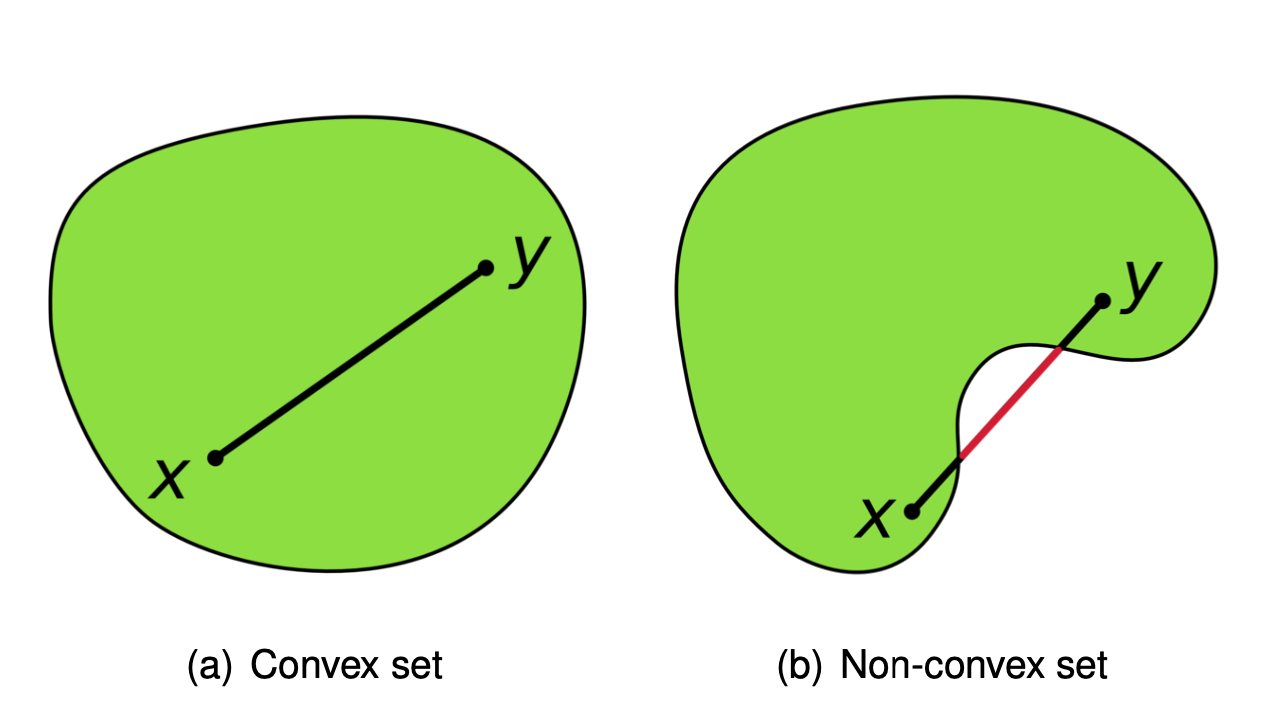
\includegraphics[scale=0.3]{Convex_set.png}
    \caption{Convex Set}
    \label{}
\end{figure}\end{center}

\begin{example}
Given $\vec{a}\in \mathbb{R}^n$ and $b\in \mathbb{R}$, the half spaces are convex
\begin{equation}
    \begin{aligned}
        \{\vec{x}\in \mathbb{R}^n: \vec{a}\vec{x}\geq b\}&\text{ (closed half-space)}\\
        \{\vec{x}\in \mathbb{R}^n: \vec{a}\vec{x}> b\}&\text{ (open half-space)}\\
    \end{aligned}
    \nonumber
\end{equation}
\end{example}

\begin{example}
$B(\vec{x},r)=\{\vec{y}\in \mathbb{R}^n:\|\vec{x}-\vec{y}\|< r\}$ is convex.
\end{example}

\subsection{Prop: convex sets $e_1,e_2,...e_n$, then $\cap_{i=1}^ne_i$ is convex}
\begin{proposition}
    If $C_1,C_2$ are convex sets, then $C_1\cap C_2$ is also convex.

    (Given a collection $e$ of convex sets, $\cap e$ is also convex)
\end{proposition}

\section{Convex Hull}
\begin{definition}[Convex Combinations]
A Convex Combination of $x_1,x_2,...,x_n\in \mathbb{R}^n$ is a linear combination $$\sum_{i=1}^k\lambda_ix_i\text{, such that }\sum_{i=1}^k\lambda_i=1,\lambda_i\geq 0,i=1,...,k$$
\end{definition}

\subsection{Convex Hull $conv(S)$ is the set of all convex combinations of points in $S$}
\begin{definition}[Convex Hull]
Given a set of points $S\subseteq \mathbb{R}^n$, the \textbf{convex hull} $conv(S)$ is the set of all convex combinations of points in $S$.

(Equivalencies: We can define the $conv(S)$ as the smallest convex set contains $S$)
\end{definition}

\subsection{Theorem: convex combination of elements in convex set is also in convex set}
\begin{theorem}
Consider a convex set $S$ and points $x_1,x_2,...,x_k\in S$, any convex combination $\lambda_1 x_1+\cdots+\lambda_k x_k$ is also in $S$
\end{theorem}
\begin{proof}
prove by induction. (Convex combination of any number points can be rewritten to a convex combination of two points.)
\end{proof}

\subsection{Corollary: $conv(S)$ is the smallest convex set containing $S$}
\begin{corollary}
    $conv(S)$ is the smallest convex set containing $S$.
\end{corollary}

\section{Optimization over Convex Set}
$$\min_{x\in \&} f(x)$$
where $\&$ is a non-empty closed and convex subset of $\mathbb{R}^n$.

Assume $f$ is continuously differentiable on $\&$.

\begin{definition}
$x^*$ is a \underline{local min of $f$ over $\&$} if $\exists \varepsilon>0$ s.t. $f(x^*)\leq f(x)\quad \forall x\in \&$ with $\|x-x^*\|<\varepsilon$.

$x^*$ is \underline{global min of $f$ over $\&$} if $f(x^*)\leq f(x)\quad \forall x\in \&$.
\end{definition}


\section{Convex Function}
\subsection{Definition: $f$ is convex $\Leftrightarrow$ $f(\alpha x+(1-\alpha) y) \leq \alpha f(x)+(1-\alpha) f(y), \forall x, y \in C, \forall \alpha \in[0,1]$}
\begin{center}
    \fcolorbox{black}{gray!10}{\parbox{.9\linewidth}{\underline{\textbf{Convex function} (0-th order)}: $f$ is \textbf{convex} in a convex set $C$ iff $f(\alpha x+(1-\alpha) y) \leq \alpha f(x)+(1-\alpha) f(y), \forall x, y \in C, \forall \alpha \in[0,1] .$ $f$ is \textbf{strictly convex} in a convex set $C$ iff $f(\alpha x+(1-\alpha) y) < \alpha f(x)+(1-\alpha) f(y), \forall x\neq y \in C, \forall \alpha \in[0,1] .$
    
    Alternative definitions of \underline{\textbf{convex function}} $f$:
    \begin{enumerate}[(1)]
        \item (differentiable): $f(z) \geq f(x)+(z-x)^{T} \nabla f(x), \ \forall x, z \in C .$
        \item (twice differentiable): $\nabla^{2} f(x) \succeq 0,\ \forall x \in C .$ ($C$ is open)
    \end{enumerate}
    }}
\end{center}

A function $f$ is a \underline{\textbf{concave function}} \underline{if and only if} $-f$ is a convex function.

\subsection{First-order: $f$ is convex $\Leftrightarrow$ $f(z) \geq f(x)+(z-x)^{T} \nabla f(x), \forall x, z \in C$}
\textbf{Alternative 1 ($1^{st}$ order)}: If $f$ is differentiable, then $f$ is convex \textbf{iff} $f(z) \geq f(x)+(z-x)^{T} \nabla f(x), \ \forall x, z \in C .$ The inequality is strict for strict convexity.
\begin{proof}
\quad
\begin{enumerate}[(i)]
    \item "$\Rightarrow$" \begin{equation}
        \begin{aligned}
            f(x+\alpha (y-x))&\leq (1-\alpha)f(x)+\alpha f(y), \forall \alpha \in (0,1)\\
            \Rightarrow	\frac{f(x+\alpha(y-x))-f(x)}{\alpha}&\leq f(y)-f(x)\\
            \text{Limit as }\alpha \rightarrow 0 \Rightarrow (y-x)^{T} \nabla f(x)&\leq f(y)-f(x)
        \end{aligned}
        \nonumber
    \end{equation}
    \item "$\Leftarrow$" Let $g=\alpha x+(1-\alpha) y$
    \begin{equation}
        \begin{aligned}
            f(g)+(x-g)^{T} \nabla f(g)&\leq f(x)\\
            f(g)+(y-g)^{T} \nabla f(g)&\leq f(y)\\
            \Rightarrow	f(g)&\leq \alpha f(x)+(1-\alpha)f(y)\\
            f(\alpha x+(1-\alpha) y)&\leq \alpha f(x)+(1-\alpha)f(y)
        \end{aligned}
        \nonumber
    \end{equation}
\end{enumerate}
\end{proof}

\subsection{Prop: local-min$\Rightarrow\nabla f(x^*)^T(x-x^*)\geq 0,\forall x\in \&$ $\Leftrightarrow$ global-min in convex }
\begin{proposition}[optimality conditions]
    \quad
    \begin{enumerate}[(a)]
        \item (Necessary Conditions for local-min) If $x^*$ is a local min of $f$ over $\&$, then $$\nabla f(x^*)^T(x-x^*)\geq 0\quad \forall x\in \&$$
        \item (Sufficient and Necessary Condition for global-min of convex $f$) If $f$ is convex over $\&$, then above condition is also sufficient for $x^*$ to be a global-min.
    \end{enumerate}
\end{proposition}
\begin{proof}
    \quad
\begin{enumerate}[(a)]
    \item Suppose $x^*$ is a local-min, and $\nabla f(x^*)^T(x-x^*)<0$ for some $x\in \&$.
    
    Let $g(\varepsilon)=f(x^*+\varepsilon(x-x^*))$, then $g'(\varepsilon)=\nabla f(x^*+\varepsilon(x-x^*))^T(x-x^*)$.
    
    By MVT(middle value theorem), $g(\varepsilon)=g(0)+\varepsilon g'(\beta\varepsilon)$ for some $\beta\in[0,1]$
    $$\Rightarrow f(x^*+\varepsilon(x-x^*))=f(x^*)+\varepsilon\nabla f(x^*+\beta\varepsilon(x-x^*))^T(x-x^*)\quad \text{for some }\beta\in[0,1]$$
    Since $\nabla f$ is continuous, we have that for all sufficient small $\varepsilon>0$, $\nabla f(x^*+\beta\varepsilon(x-x^*))^T(x-x^*)<0 \Rightarrow f(x^*+\varepsilon(x-x^*))=f(x^*)$

    Since $x^*+\varepsilon(x-x^*)=\varepsilon x+(1-\varepsilon)x^*\in \&$, then $x^*$ can't be a local-min over $\&$ $\rightarrow$ contradiction.
    \item Convexity of $f$ over $\&$ $\Rightarrow f(x)\geq f(x^*)+\nabla f(x^*)^T(x-x^*),\quad \forall x\in \&$.
    
    Thus,
    \begin{equation}
        \begin{aligned}
            &\nabla f(x^*)^T(x-x^*),\quad \forall x\in \&\\
            \Rightarrow	& f(x)\geq f(x^*)\quad \forall x\in \&\\
            \Rightarrow	& x^*\text{ is a global min of $f$ over }\&
        \end{aligned}
        \nonumber
    \end{equation}
\end{enumerate}
\end{proof}

\textbf{Example:}
\begin{align*}
    &\max_{x\in\&}\quad x_1^{a_1}x_2^{a_2}\cdots x_n^{a_n}\\
    &\begin{array}{r@{\quad}r@{}l@{\quad}l}
    &\&=\{x:\sum_{i=1}^nx_i=1,x_i\geq 0,i=1,2,...,n\} &\\
    &a_i,i=1,2,...,n \text{ are given positive scalars}&\\
\end{array} .
\end{align*}
Equivalent to $$\min_{x\in\&}\quad f(x)$$ with $f(x)=-\sum a_i\ln x_i$
\begin{equation}
    \begin{aligned}
        \nabla f(x)&=\left(-\frac{a_1}{x_1},-\frac{a_2}{x_2},...,-\frac{a_n}{x_n}\right)\\
        \nabla^2 f(x)&=diag\left(\frac{a_1}{x^2_1},\frac{a_2}{x^2_2},...,\frac{a_n}{x^2_n}\right)\succ 0\\
        &\Rightarrow f\text{ is strictly convex}.
    \end{aligned}
    \nonumber
\end{equation}
\begin{equation}
    \begin{aligned}
        x^*\in\&\text{ is (unique) min}&\Leftrightarrow \nabla f(x^*)^T(x-x^*)\geq 0\quad \forall x\in\&.\\
        &\Leftrightarrow -\sum_{i=1}^n\frac{a_i}{x_i^*}(x-x^*)\geq 0\quad \forall x\in\&.\\
        &\Leftrightarrow -\sum_{i=1}^na_i\frac{x_i}{x_i^*}+\sum_{i=1}^na_i\geq 0\quad \forall x\in\&.\\
    \end{aligned}
    \nonumber
\end{equation}
Guess: $x^*_i=\frac{a_i}{\sum_{i=1}^na_i}$. Then,
\begin{equation}
    \begin{aligned}
        -\sum_{i=1}^n a_i\frac{x_i}{x_i^*}+\sum_{i=1}^na_i=0,\quad \forall x\in\&
    \end{aligned}
    \nonumber
\end{equation}
Thus $x^*=\frac{a_i}{\sum_{i=1}^na_i}$ is unique min.


\subsection{Second-order: $f$ is convex $\Leftrightarrow$ $\nabla^{2} f(x) \succeq 0,\ \forall x \in C$}
\textbf{Alternative 2 ($2^{nd}$ order)}: If $f$ is twice differentiable and $C$ is open and convex, then $f$ is convex iff
$$
\nabla^{2} f(x) \succeq 0,\ \forall x \in C
$$
\begin{proof}
    \begin{enumerate}
        \item[$\Rightarrow$]: Suppose $f:C \rightarrow \mathbb{R}$ is convex and take $x^*\in C$. Define $g: C \rightarrow \mathbb{R}$ as $g(y)=f(y)-(y-x^*)\nabla f(x^*)$. Because $g$ is a sum of convex functions ($f(y)$ and $-(y-x^*)\nabla f(x^*)$ which is linear), $g$ is convex.
        
        Because $\nabla g(y)=\nabla f(y)-\nabla f(x^*)$, $x^*$ is the critical point of $g$, $x^*$ is the global min of $g$. We can also show $Hg(y)=Hf(y)$. If $Hg(x^*)=Hf(x^*)$ is not positive semidefinite, then we had a negative eigenvalue $u$ s.t. $g(x^*+tu)$ is decreasing in $t$ s.t. $x^*$ is not a global minimizer of $g$, contradiction. Since $x^*$ is arbitrary, $Hg(x^*)\succeq 0,\forall x^*\in C$.
        \item[$\Leftarrow$]: \textbf{Taylor:} Given a function $f:\mathbb{R}^n \rightarrow \mathbb{R}$, if $Hf$ is continuous and $\vec{x}^*$ is a critical point of $f$, then
        $$f(\vec{x})=f(\vec{x}^*)+\nabla f(\vec{x}^*)(\vec{x}-\vec{x}^*)+\frac{1}{2}(\vec{x}-\vec{x}^*)^T Hf(\vec{z}) (\vec{x}-\vec{x}^*)$$
        for some $\vec{z}$ on the line between $\vec{x}$ and $\vec{x}^*$.
    \end{enumerate}
\end{proof}





\subsection{Sufficient Condition of Strictly Convex: $\nabla^{2} f(x) \succ 0$}
Strictly convex: $\nabla^{2} f(x) \succ 0,\ \forall x \in C \text{ ($C$ is open)} \Rightarrow	$ $f$ is strictly convex.


\textbf{Note:} $f$ is strictly convex $\nRightarrow \nabla^{2} f(x) \succ 0$.
\begin{example}
$f(x)=x^4\text{(strictly convex)}$, $\frac{d^2f(x)}{dx^2}=12x^2(=0\text{ at }x=0)$
\end{example}


\subsection{Prop: Max and Linear combination of convex functions are also convex}
\textbf{Properties: }Convex functions $f$ over $\mathbb{R}^n$, $\{f_i\}_{i\in \mathbb{Z}}$ over $\&$:
\begin{enumerate}[(1)]
    \item $C=\{x\in \mathbb{R}^n| f(x)\leq a\}$ is convex set, $\forall a\in \mathbb{R}$.
    \item Suppose $\{f_i\}_{i\in \mathbb{Z}}$ are convex functions $C \rightarrow \mathbb{R}$. $\alpha_1,\alpha_2,...,\alpha_k$ are positive scalars, then $$f_{sum}(x)=\sum_{i=1}^k\alpha_if_i(x)$$ is convex. If at least on $f_i$ is strictly convex, $f_{sum}$ is strictly convex.
    \item $f_{max}(x)=\max_{i=1,...,k}f_i(x)$ is convex over $\&$ (strictly convex if all $f_i$ are strictly convex)
\end{enumerate}
\begin{proof} Prove (2) here:\\
    We need to show (1) $\alpha f_i$ is convex; (2) $H(x)=f_1(x)+f_2(x)$ is convex and strictly convex if one is strictly convex.

    (1): can be proved by definition.\\
    (2): $H(\lambda x+(1-\lambda)y)=f_1(\lambda x+(1-\lambda)y)+f_2(\lambda x+(1-\lambda)y)\leq \lambda (f_1(x)+f_2(x))+(1-\lambda)(f_1(y)+f_2(y))=\lambda H(x)+(1-\lambda)H(y),\lambda\in [0,1]$ $\Rightarrow$ $H$ is convex. (We can get strict inequality if one is strictly convex).
\end{proof}
\begin{proof} Prove (3) here:
\begin{equation}
    \begin{aligned}
        f_{max}(\alpha x+(1-\alpha)y)&=\max_{i=1,...,k}f_i(\alpha x+(1-\alpha)y)\\
    &\leq \max_{i=1,...,k}[\alpha f_i(x)+(1-\alpha)f_i(y)]\\
    &\leq \max_{i=1,...,k}\alpha f_i(x)+\max_{i=1,...,k}(1-\alpha)f_i(y)\\
    &=\alpha f_{max}(x)+(1-\alpha)f_{max}(y)
    \end{aligned}
    \nonumber
\end{equation}
Inequality is strict if all $f_i$ are strictly convex.
\end{proof}



\section{Lemma: function $f$ is a convex function iff $\phi(t)=f(\vec{x}+t\vec{u})$ is convex of $t$}
\begin{lemma}
    Let $C\subseteq \mathbb{R}^n$ be a convex set. A function $C \rightarrow \mathbb{R}$ is convex if and only if, for all $\vec{x}\in C$ and $\vec{u}\in \mathbb{R}^n$, the function $$\phi(t)=f(\vec{x}+t\vec{u})$$ is a single-variable convex function of $t$.
\end{lemma}

\section{Proposition: Convex function $f$, $\nabla f(x^*)=0$ $\Rightarrow$ global-min}
\begin{proposition}
    Let $f: X \longmapsto \mathbb{R}$ be a convex function over the convex set $X$.

    (a) A local-min of $f$ over $X$ is also a global-min over $X$. If $f$ is strictly convex, then min is unique.

    (b) If $X$ is open (e.g. $\mathbb{R}^{n}$ ), then $\nabla f\left(x^{*}\right)=0$ is a necessary and sufficient condition for $x^{*}$ to be a global minimum.
\end{proposition}
\begin{proof}
\quad\\
Proof based on a property: If $f$ is differentiable over $C$ (open), then $f$ is convex iff
$$
f(z) \geq f(x)+(z-x)^{\prime} \nabla f(x), \quad \forall x, z \in C .
$$
\end{proof}


\begin{corollary}
    Let $f: X \longmapsto \mathbb{R}$ be a concave function over the convex set $X$.

    (a) A local-max of $f$ over $X$ is also a global-max over $X$.

    (b) If $X$ is open (e.g. $\mathbb{R}^{n}$ ), then $\nabla f\left(x^{*}\right)=0$ is a necessary and sufficient condition for $x^{*}$ to be a global maximum.
\end{corollary}





\section{Application: Unconstrained Quadratic Optimization}
$$\begin{array}{ll}\text { minimize } & f(\mathbf{w})=\frac{1}{2} \mathbf{w}^{T} \mathbf{Q} \mathbf{w}-\mathbf{b}^{T} \mathbf{w} \\ \text { subject to } & \mathbf{w} \in \mathbb{R}^{d}\end{array}$$
where $\mathbf{Q}$ is a symmetric $d \times d$ matrix. (what if non-symmetric?)
$$\nabla f(\mathbf{w})=\mathbf{Q}\mathbf{w}-\mathbf{b},\ \nabla^2 f(\mathbf{w})=\mathbf{Q}$$
\begin{enumerate}[(i)]
    \item $\mathbf{Q}\succeq 0 \Leftrightarrow	f$ is convex.
    \item $\mathbf{Q}\succ 0 \Leftrightarrow	f$ is strictly convex.
    \item $\mathbf{Q}\preceq 0 \Leftrightarrow	f$ is concave.
    \item $\mathbf{Q}\prec 0 \Leftrightarrow	f$ is strictly concave.
\end{enumerate}









- Necessary condition for (local) optimality
$$
\mathbf{Q} \mathbf{w}=\mathbf{b}, \quad \mathbf{Q} \succeq 0
$$

Case 1: $\mathbf{Q w}=\mathbf{b}$ has no solution, i.e. $\mathbf{b} \notin R(\mathbf{Q})$. No stationary point, no lower bound ($f$ can achieve $-\infty$).

Case 2: $\mathbf{Q}$ is not PSD ( $f$ is non-convex)
No local-min, no lower bound ($f$ can achieve $-\infty$).

Case 3: $\mathbf{Q} \succeq 0$ (PSD) and $\mathbf{b} \in R(\mathbf{Q})$. Convex, has global-min, 
any stationary point is a global optimal solution.

\begin{example}
    Toy Problem 1: $\min _{x, y \in \mathbb{R}} f(x, y) \triangleq x^{2}+y^{2}+\alpha x y$.
\end{example}
\begin{enumerate}
    \item Step 1: First order condition: $2 x^{*}+\alpha y^{*}=0,2 y^{*}+\alpha x^{*}=0$.
    
    - We get $4 x^{*}=-2 \alpha y^{*}=\alpha^{2} x^{*}$. So $\left(4-\alpha^{2}\right) x^{*}=0$.
    
    - Case 1: $\alpha^{2}=4$. If $x^{*}=-\alpha y^{*} / 2$, then $\left(x^{*}, y^{*}\right)$ is a stationary point.
    
    - Case 2: $\alpha^{2} \neq 4$. Then $x^{*}=0 ; y^{*}=-\alpha x^{*} / 2=0$. So $(0,0)$ is stat-pt.
    \item Step 2: Check convexity. Hessian $\nabla^{2} f(x, y)=\left(\begin{array}{ll}2 & \alpha \\ \alpha & 2\end{array}\right)$.
    
    Eigenvalues $\lambda_{1}, \lambda_{2}$ satisfy $\left(\lambda_{i}-2\right)^{2}=\alpha^{2}, i=1,2$.
    Thus $\lambda_{1,2}=2 \pm|\alpha|$.

    - If $|\alpha| \leq 2$, then $\lambda_{i} \geq 0, \forall i$. Thus $f$ is convex. Any stat-pt is global-min.

    - If $|\alpha|>2$, at least one $\lambda_{i}<0$, thus $f$ is not convex.
    \item Step 3 (can be skipped now): For non-convex case $(|\alpha|>2)$, prove no lower bound.
    
    $f(x, y)=(x+\alpha y / 2)+\left(1-\alpha^{2} / 4\right) y^{2}$. Pick $y=M, x=-\alpha M / 2$, then
    $f(x, y)=\left(1-\alpha^{2} / 4\right) M^{2} \rightarrow-\infty$ as $M \rightarrow \infty$.
\end{enumerate}

Summary:

If $|\alpha|>2$, no global-min, $(0,0)$ is stat-pt;

if $|\alpha|=2$, any $(-0.5 \alpha t, t), t \in \mathbb{R}$ is a stat-pt and global-min;

if $|\alpha|<2,(0,0)$ is the unique stat-pt and global-min.

\begin{example}
Linear Regression
\end{example}
$\text{minimize } f(\mathbf{w})=\frac{1}{2}\left\|\vec{x}^{T} \mathbf{w}-\vec{y}\right\|^{2}$ subject to $ \mathbf{w} \in \mathbb{R}^{d}$

$n$ data points, $d$ features

- $\vec{x}$ may be wide (under-determined), tall (over-determined), or rank-deficient

- Note that comparing with the previous case, $\mathbf{Q}=\mathbf{X X}^{T} \in \mathbb{R}^{d \times d}$, $\mathbf{b}=\vec{x} \vec{y} \in \mathbb{R}^{d \times 1}$

- $\mathbf{Q} \succeq 0$; Case 2 never happens!

- First order condition $\mathbf{X X}^{\top} \mathbf{w}^{*}=\vec{x} \vec{y}$.

\quad - It always has a solution; Case 1 never happens!

\begin{claim}
    Linear regression problem is always convex; it has global-min.
\end{claim}
$$
\mathbf{X X}^{\top} \mathbf{w}^{*}=\vec{x} \vec{y}
$$
which always has a solution.

If $X X^{\top} \in \mathbb{R}^{d \times d}$ is invertible (only happen when $n \geq d$ ), then there is a unique stationary point $x=\left(A^{\top} A\right)^{-1} A^{\top} b$. It is also a global minimum.

If $X X^{\top} \in \mathbb{R}^{d \times d}$ is not invertible, then there can be infinitely many stationary points, which are the solutions to the linear equation.
All of them are global minima, giving the same function value.



\section{Theorem: If $f$ is convex and $g$ is convex and increasing, $(g\cdot f)(x)$ is convex}
\begin{theorem}
    If $f$ is convex and $g$ is convex and increasing, $(g\cdot f)(x)=g(f(x))$ is convex. Moreover, if $f$ is strictly convex and $g$ is strictly increasing $g\cdot f$ is strictly convex.
\end{theorem}
\begin{proof}
$g(f(\lambda x+(1-\lambda)y))\leq g(\lambda f(x)+(1-\lambda) f(y))\leq \lambda g(f(x))+(1-\lambda)g(f(y))$ (the first inequality is strict when $f$ is strictly convex and $g$ is strictly increasing)
\end{proof}
\begin{corollary}
    $f(x)=|x|^p,p\geq 1$ is convex. ($f_1(x)=|x|$ is convex in $\mathbb{R}$, $f_2(x)=x^p,p\geq 1$ is convex in $\mathbb{R}^+\cup\{0\}$)
\end{corollary}
Except proving $f(x)=|x|^p,p\geq 1$ is convex we can also prove $f(x)=|x|^p,p\in(1,2]$ is strongly convex in $[-1,1]$.
\begin{corollary}
    $f(x)=|x|^p,p\in(1,2]$ is strongly convex in $[-1,1]$.
\end{corollary}
\begin{proof}
$F(x)=f(x)-mx^2=|x|^p-\frac{m}{2}x^2$. $g_1(x)=|x|,x\in [-1,1]$ is convex; We want to prove $g_2(x)=x^p-\frac{m}{2}x^2,x\in [0,1]$ is also convex:
\begin{enumerate}[(1)]
    \item $p= 2$ ($g_2$ is twice differentiable): $g_2^{''}(x)=p(p-1)-m\geq 0$ for $m\leq p(p-1)$ $\Rightarrow$ $g_2(x)$ is convex and increasing in $[0,1]$.
    \item $p\in (1,2)$ ($g_2$ is not twice differentiable at $0$): $g_2^{'}(x)=px^{p-1}-mx$. Let
    \begin{equation}
        \begin{aligned}
            G_x(y)&=g_2(y)+(x-y)g_2^{'}(y),\ y\in [0,1]\\
            \frac{\partial G_x(y)}{\partial y}&=xg^{''}_2(y)-yg^{''}_2(y)=(x-y)g^{''}_2(y)\\
            &=\left(p(p-1)y^{p-2}-m\right)(x-y),\ y\in(0,1]
        \end{aligned}
        \nonumber
    \end{equation}
    for $m\leq p(p-1)$, $\frac{\partial G_x(y)}{\partial y}\geq 0, y\in (0,x]$ and $\frac{\partial G_x(y)}{\partial y}\leq 0, y\in [x,1]$.

    Then $G_x(y)\leq G_x(x),\forall y\in (0,1]$

    $G_x(0)=0$, $G_x(x)=g_2(x)=x^p-\frac{m}{2}x^2$. Since we know $g_2(x)\geq 0,\forall x\in [0,1]$ if $m\leq 2$, we can infer $G_x(y)\leq g_2(x)$. i.e., $g_2(y)+(x-y)g_2^{'}(y)\leq g_2(x),\forall x,y\in [0,1]$. Then we can infer $g_2(x)$ is convex and increasing for $m<p(p-1)$.
\end{enumerate}
\end{proof}

\section{Corollary: $f$ is linear, $g$ is convex (not necessarily increasing) $\Rightarrow$ $g\cdot f$ is convex}
\begin{corollary}
    Suppose $f:\mathbb{R}^m \rightarrow \mathbb{R}^n$ with $f(x)=Ax+b$ and $g:C \rightarrow \mathbb{R}$ is convex, then $h(x)=g(f(x))$ is convex as function $f^{-1}(C) \rightarrow \mathbb{R}$.
\end{corollary}
\begin{proof}
For $\lambda\in[0,1]$,
\begin{equation}
    \begin{aligned}
        h(\lambda x+(1-\lambda)y)&=g(f(\lambda x+(1-\lambda)y))= g(\lambda(Ax+b)+(1-\lambda)(Ay+b))\\
        &\leq \lambda g(Ax+b)+(1-\lambda)g(Ay+b)=\lambda h(x)+(1-\lambda)h(y)
    \end{aligned}
    \nonumber
\end{equation}
\end{proof}


\begin{example}
    Prove $f(x,y,z)=(\frac{x}{2})^x(\frac{y}{3})^y(\frac{z}{4})^z$ is convex on $\{x>0,y>0,z>0\}$
\end{example}
We can rewrite the function
\begin{equation}
    \begin{aligned}
        f(x,y,z)=e^{x\ln(\frac{x}{2})+y\ln(\frac{y}{3})+z\ln(\frac{z}{4})}=g(h(x,y,z))
    \end{aligned}
    \nonumber
\end{equation}
where $h(x,y,z)=x\ln(\frac{x}{2})+y\ln(\frac{y}{3})+z\ln(\frac{z}{4})$ and $g(x)=e^x$.

$\frac{\partial^2 x\ln(\frac{x}{c})}{\partial x^2}=\frac{1}{x}>0$ $\Rightarrow$ $h(x,y,z)$ is convex. And we can check $g(x)$ si convex and increasing. We can know $f(x,y,z)$ is convex.

\section{Epigraph and Jensen's Inequality}
\subsection{Def: epigraph ${epi}(f)=\{(x,y)\in C\times \mathbb{R}:y\geq f(x)\}$}
\begin{definition}
    Given a subset $C \subseteq \mathbb{R}^n$ and a function $f: C \rightarrow \mathbb{R}$, the \textbf{epigraph} of $f$ is a set $${epi}(f)=\{(x,y)\in C\times \mathbb{R}:y\geq f(x)\}$$
\end{definition}

\subsection{Lemma: $f$ is convex function $\Leftrightarrow$ ${epi}(f)$ is a convex set}
\begin{lemma}
    Consider some $f: C \rightarrow \mathbb{R}$ where $C\subseteq \mathbb{R}^n$ is a convex set. Then $f$ is a convex function \textbf{iff} ${epi}(f)$ is a convex set.
\end{lemma}
\begin{proof}
Prove $\Rightarrow$: Suppose $f$ is a convex set and for any points in $epi(f)$, $(x_1,y_1),(x_2,y_2)\in epi(f)$.
\begin{equation}
    \begin{aligned}
        \lambda y_1+(1-\lambda)y_2\geq \lambda_1f(x_1)+(1-\lambda)f(x_2)\geq f(\lambda x_1+(1-\lambda)x_2)
    \end{aligned}
    \nonumber
\end{equation}
($\lambda\in[0,1]$)
By definition $\Rightarrow$ $\lambda y_1+(1-\lambda)y_2$ is also in ${epi}(f)$ $\Rightarrow$ ${epi}(f)$ is a convex set.

Prove $\Leftarrow$: Suppose ${epi}(f)$ is a convex set. For $x_1,x_2\in C$, by definition $(x_1,f(x_1)),(x_2,f(x_2))\in {epi}(f)$. Then $(\lambda x_1+(1-\lambda)x_2,\lambda f(x_1)+(1-\lambda)f(x_2))\in {epi}(f)$ $\Rightarrow$ $\lambda f(x_1)+(1-\lambda)f(x_2))\geq f(\lambda x_1+(1-\lambda)x_2)$ $\Rightarrow$ $f$ is convex.
\end{proof}

\subsection{Jensen's Inequality: $f(\sum_{i=1}^k\lambda_i x_i)\leq \sum_{i=1}^k\lambda_if(x_i)$}
\begin{theorem}[Jensen's Inequality]
    For any $\lambda_i\geq 0,i=1,...,k$ and $\sum_{i=1}^k\lambda_i=1$, if $f: C \rightarrow \mathbb{R}$ is convex and $\{x_i,i=1,...,k\}$ is a collection of points in $C$, then $$f(\sum_{i=1}^k\lambda_i x_i)\leq \sum_{i=1}^k\lambda_if(x_i)$$
\end{theorem}

Note: If $f$ is strictly convex and $\lambda_i>0,\forall i$, then $f(\sum_{i=1}^k\lambda_i x_i)= \sum_{i=1}^k\lambda_if(x_i)$ iff $x_1=x_2=\cdots=x_k$.
\begin{proof}
    For each $\vec{x}_1,...,\vec{x}_k$, there is a corresponding point $(\vec{x}_1,f(\vec{x}_1)),(\vec{x}_2,f(\vec{x}_2)),...,(\vec{x}_k,f(\vec{x}_k))\in {epi}(f)$. Because ${epi}(f)$ is convex,
    \begin{equation}
        \begin{aligned}
            \lambda_1 \begin{bmatrix}
                \vec{x}_1\\
                f(\vec{x}_1)
            \end{bmatrix}+\cdots+\lambda_k \begin{bmatrix}
                \vec{x}_k\\
                f(\vec{x}_k)
            \end{bmatrix}\in {epi}(f)
        \end{aligned}
        \nonumber
    \end{equation}
    i.e. $\begin{bmatrix}
        \lambda_1\vec{x}_1+\cdots+\lambda_k\vec{x}_k\\
        \lambda_1f(\vec{x}_1)+\cdots+\lambda_kf(\vec{x}_k)
    \end{bmatrix}\in{epi}(f)$. This means that $$\lambda_1f(\vec{x}_1)+\cdots+\lambda_k f(\vec{x}_k)\geq f(\lambda_1\vec{x}_1+\cdots+\lambda_k\vec{x}_k)$$
\end{proof}

\section{Subgradients of Convex Functions}
Consider convex functions that are unlikely to be differentiable everywhere.
\subsection{Sub-gradient $\vec{d}$: $f(\vec{x})\geq f(\vec{x}^*)+\vec{d}\cdot (\vec{x}-\vec{x}^*), \forall \vec{x}\in C$}
\begin{lemma}
    If $C\subseteq \mathbb{R}^n$ is a convex set, $f: C \rightarrow  \mathbb{R}$ is a convex function, and $\vec{x}^*\in int(C)$, then there exists some vector $\vec{d}\in \mathbb{R}^n$ such that $$f(\vec{x})\geq f(\vec{x}^*)+\vec{d}\cdot (\vec{x}-\vec{x}^*),\ \forall \vec{x}\in C$$
\end{lemma}
\begin{definition}
    The $\vec{d}$ satisfied the inequality is called a \textbf{sub-gradient} of $f$ at $\vec{x}^*$.
\end{definition}
\begin{proof}
    We can use epigraphs. Recall that for a function $f: C \rightarrow \mathbb{R}$, $$epi(f)=\{(\vec{x},y)\in \mathbb{R}^{n+1}: y\geq f(\vec{x})\}$$
    when $C$ is a convex set and $f$ is a convex function, $epi(f)$ is a convex set.\\
    Choose $\vec{x}^*\in int(C)$, then $\left(\vec{x}^*,f(\vec{x}^*)\right)$ is a boundary point of $epi(f)$.\\
    By the support theorem, there exists a vector $(\vec{a},b)\in \mathbb{R}^{n+1}$ with $\|(\vec{a},b)\|=1$ such that
    \begin{equation}
        \begin{aligned}
            (\vec{a},b)\cdot \left(\vec{x}^*,f(\vec{x}^*)\right)&\geq (\vec{a},b)\cdot \left(\vec{x},y\right)\\
            \vec{a}\cdot \vec{x}^*+ b f(\vec{x}^*)&\geq \vec{a}\cdot \vec{x}+ by,\ \forall \left(\vec{x},y\right)\in epi(f)
        \end{aligned}
        \nonumber
    \end{equation}
    Specifically, we substitute $(\vec{x}^*,f(\vec{x}^*)+\varepsilon)\in epi(f)$ into the inequality, where $\varepsilon\geq 0$, $b\varepsilon\leq 0$ $\Rightarrow b\leq 0$.\\
    If $b=0$, $\vec{a}\cdot \vec{x}^*\geq \vec{a}\cdot \vec{x},\forall \vec{x}\in C$. By the separation theorem and $\vec{x}^*\in int(C)$, we can there must exist $\vec{y}\in C$ such that $\vec{a}\cdot \vec{y}>\vec{a}\cdot \vec{x}^*$ which contradicts to the inference. Hence, $b>0$.\\
    Substitute the form $(\vec{x},f(\vec{x}))$,
    \begin{equation}
        \begin{aligned}
            \vec{a}\cdot \vec{x}^*+ b f(\vec{x}^*)&\geq \vec{a}\cdot \vec{x}+ bf(\vec{x})\\
            bf(\vec{x})&\leq bf(\vec{x}^*)-\vec{a}(\vec{x}-\vec{x}^*)
        \end{aligned}
        \nonumber
    \end{equation}
    Since $b<0$, we can divide the equation by $b$ on each side:
    \begin{equation}
        \begin{aligned}
            f(\vec{x})&\geq f(\vec{x}^*)-\frac{\vec{a}}{b}(\vec{x}-\vec{x}^*)
        \end{aligned}
        \nonumber
    \end{equation}
    The set of all available $-\frac{\vec{a}}{b}$ are the sub-gradient we want.
\end{proof}
\subsection*{\underline{Properties of Sub-gradient}}
\begin{enumerate}[1)]
    \item Sub-gradient always exist at any point for convex functions.
    \item If $\nabla f$ exists at a point $x$ for convex $f$ $\Leftrightarrow$ Sub-gradient is \underline{unique and $=\nabla f(x)$}
    \item Some definition for sub-gradient can be applied for non-convex $f$, but sub-gradient may not exist.
\end{enumerate}

\begin{example}
$f(x)=|x|,x\in \mathbb{R}$
\end{example}
For $x\neq 0$, $\nabla f$ exists and $=$ sub-gradient.\\
For $x=0$, any $g\in[-1,1]$ is a sub-gradient.
\begin{proof}\quad
\begin{enumerate}[(1)]
    \item For $y>0$, $f(y)=y\geq f(0)+gy=gy,\forall g\in[-1,1]$
    \item For $y<0$, $f(y)=-y\geq f(0)+gy=gy,\forall g\in[-1,1]$
\end{enumerate}
\end{proof}

\subsection{Sub-differential: set of all sub-gradient}
\begin{definition}
    Set of all sub-gradient of $f$ at $\vec{x}^*$ is called \textbf{sub-differential} of $f$ at $\vec{x}^*$, denoted $\partial f(\vec{x}^*)$.
\end{definition}
\begin{example}
For $f(x)=|x|$,
\begin{equation}
    \begin{aligned}
        \partial f(x)=\left\{\begin{matrix}
            -1&\text{ if }x<0\\
            [-1,1]&\text{ if }x=0\\
            1&\text{ if }x>0\\
        \end{matrix}\right.
    \end{aligned}
    \nonumber
\end{equation}
\end{example}

\begin{example}
For $f(x)=\max\{1,|x|-1\}$. (Note: $f(x)$ is convex since $1,|x|-1$ are both convex.)
\begin{equation}
    \begin{aligned}
        \partial f(x)=\left\{\begin{matrix}
            -1&\text{ if }x<-2\\
            [-1,0]&\text{ if }x=-2\\
            0&\text{ if }-1<x<2\\
            [0,1]&\text{ if }x=2\\
            1&\text{ if }x>2\\
        \end{matrix}\right.
    \end{aligned}
    \nonumber
\end{equation}
\end{example}
When $x=2$,
\begin{equation}
    \begin{aligned}
        f(y)=\max\{1,|y|-1\}\geq f(2)+g(y-2)=1+g(y-2)
    \end{aligned}
    \nonumber
\end{equation}
\begin{enumerate}[(1)]
    \item \underline{$y\geq 0$}: $0\geq g(y-2)$ or $0\geq (g-1)(y-2)$. If $y>2$, $g\leq 1$; If $y=2$, $\forall g$; If $0\leq y< 2$, $g\geq 0$. $\Rightarrow g\in[0,1]$
    \item \underline{$y< 0$}: $0\geq g(y-2)$ or $-y-2\geq g(y-2)$, i.e. $g\geq 0$ or $g\leq \frac{2+y}{2-y}$ (satisfied by $g\in[0,1]$)
\end{enumerate}

\subsection{More examples}
\begin{example}
    $f(x)=-\sqrt{x},\ x\in C=[0,\infty)$
\end{example}
It does not have a sub-gradient at $x^* = 0$, because the only possible tangent line is vertical. This shows that the hypothesis $x^*\in int(C)$ is necessary.




\begin{example}
    $f(x)=\|x\|=\sqrt{x^Tx}$
\end{example}
\begin{enumerate}[$\bullet$]
    \item $f$ is convex (by Triangle Inequality: $\|x\|+\|y\|\geq \|x+y\|$)
    \item For $x\neq 0$, $\nabla f(x)$ exists and $$\partial f(x)= \nabla f(x) =\frac{1}{2\sqrt{x^Tx}}\cdot 2x=\frac{x}{\|x\|}$$
    \item If $x=0$, $\nabla f(x)$ doesn't exist.
    \begin{claim}
        $\partial f(0)=\{g\in \mathbb{R}^n:\|g\|\leq 1\}$
    \end{claim}
    \begin{proof}
        Need to show that for $\|g\|\leq 1$ and $\forall y\in \mathbb{R}^n$, $$f(y)=\|y\|\geq f(0)+g^T(y-0)=g^T y$$
        But by Cauchy-Schwarz inequality, for $\|g\|\leq 1$, $$g^Ty\leq \|g\|\|y\|\leq \|y\|,\forall y\in \mathbb{R}^n$$
        To estabilish the converse, suppose $\|g\|>1$.

        Then, setting $y=\frac{g}{\|g\|}$ $\Rightarrow$ $\|y\|=1$ but $g^Ty=\|g\|>1=\|y\|$
    \end{proof}
\end{enumerate}

\begin{example}
    $f(x)=|x_1-x_2|\leftarrow$ convex
\end{example}
\begin{enumerate}[$\bullet$]
    \item If $x_1>x_2$, $|x_1-x_2|=x_1-x_2$, and $\nabla f$ exists and $(1,-1)$
    \item If $x_1<x_2$, $|x_1-x_2|=x_2-x_1$, and $\nabla f$ exists and $(-1,1)$
    \item If $x_1=x_2$,
    \begin{claim}
        If $x_1=x_2$, $\partial f(x)=\{(a,b):a=-b,|a|\leq 1\}$
    \end{claim}
    \begin{proof}
        Suppose $x_1=x_2=c$. Then we need to show $\forall y\in \mathbb{R}^2$, $(a,b)$ s.t. $a=-b$, $|a|\leq 1$
        \begin{equation}
            \begin{aligned}
                |y_1-y_2|\geq f(c,c)+[a\ b]\begin{bmatrix}
                    y_1-c\\
                    y_2-c
                \end{bmatrix}=ay_1+by_2-c(a+b)=a(y_1-y_2)
            \end{aligned}
            \nonumber
        \end{equation}
        Since $|a|<1$, this inequality holds $\forall y\in \mathbb{R}^2$
        
        To show the converse,
        \begin{enumerate}
            \item Suppose $a\neq -b$.
            
            If $c(a+b)<0$, setting $y_1=y_2=0$. $\Rightarrow |y_1-y_2|=0$, and $ay_1+by_2-c(a+b)=-c(a+b)>0=|y_1-y_2|$, above inequality fails to hold.
    
            If $c(a+b)>0$, setting $y_1=y_2=2c$. $\Rightarrow |y_1-y_2|=0$, and $ay_1+by_2-c(a+b)=c(a+b)>0=|y_1-y_2|$, above inequality fails to hold.
    
            If $c=0$, setting $y_1=y_2=(a+b)$. $\Rightarrow |y_1-y_2|=0$, and $ay_1+by_2-c(a+b)=(a+b)^2>0=|y_1-y_2|$, above inequality fails to hold.
            \item Suppose $a=-b$ with $|a|>1$.
            
            If $a>1$, setting $y_1=y_2+1$; If $a<-1$, setting $y_1=y_2-1$.
    
        \end{enumerate}
    \end{proof}
\end{enumerate}













\end{document}